\documentclass[10pt,aspectratio=169]{beamer}
\usepackage[utf8]{inputenc}
\usepackage{listings}
\usepackage{hyperref}
\usepackage{xcolor}
\usepackage{ragged2e}
\usepackage{graphicx}
\usepackage{tikz}
\usetikzlibrary{positioning,calc,decorations.pathreplacing}

\usetheme{Dresden}
%\usetheme{Bergen}

\title{Programming Techniques 2026--2027}
\author{Hannu Parviainen}
\institute{Universidad de la Laguna}
\date{\today}

% Single spaces after full stops, so that e.g. \texttt{a .dot. b} has even spacing
\frenchspacing

\lstset{
  language=fortran,
  basicstyle=\ttfamily\scriptsize,
  columns=fullflexible,
  keepspaces=true,
  backgroundcolor=\color{white},
  keywordstyle=\color{blue},
  commentstyle=\color{gray},
  stringstyle=\color{red},
  showstringspaces=false,
  breaklines=true,
  frame=lines
}

\subtitle{Lecture 10: More OpenMP: Worksharing, Synchronisation, and Performance}

\begin{document}

\begin{frame}
  \titlepage
\end{frame}


\section{Recap}

\begin{frame}[fragile]
  \frametitle{Recap: OpenMP so far}
  \begin{columns}[T]
    \begin{column}{0.58\textwidth}
      \centering
      \footnotesize
      \begin{tabular}{ll}
        \textbf{Directive or clause} & \textbf{Meaning} \\
        \hline
        \texttt{!\$omp parallel}       & start a team of threads \\
        \texttt{!\$omp do}             & share the iterations of a loop \\
        \texttt{!\$omp parallel do}    & both in one directive \\
        \texttt{shared}, \texttt{private} & one copy, or one copy per thread \\
        \texttt{firstprivate}          & private, initialised from outside \\
        \texttt{reduction(+:s)}        & private partial results, combined \\
        \texttt{collapse(2)}           & share two nested loops \\
        \texttt{!\$ }                  & compile this line only with OpenMP \\
        \texttt{omp\_get\_wtime()}     & wall-clock time, for speedups \\
        \hline
      \end{tabular}
    \end{column}

    \begin{column}{0.42\textwidth}
      \begin{lstlisting}
!$omp parallel do default(none) &
!$omp shared(x, n) private(t) &
!$omp reduction(+:s)
do i = 1, n
  t = x(i)**2
  s = s + t
end do
!$omp end parallel do
      \end{lstlisting}

      \vspace*{2mm}
      Today:
      \begin{itemize}
        \item \texttt{single}, \texttt{workshare}, \texttt{sections},
        \item barriers, \texttt{critical}, \texttt{atomic},
        \item scheduling and Amdahl's law.
      \end{itemize}
    \end{column}
  \end{columns}
\end{frame}


\section{Worksharing}

\begin{frame}
  \centering
  \Huge \textbf{More Worksharing}
\end{frame}


\begin{frame}[fragile]
  \frametitle{One parallel region instead of many}
  Forking and joining threads costs time, so it is better to have one parallel region than many. But then every thread runs the code between the loops: here, each thread updates the whole array while the others read and write it.

  \vspace*{1mm}
  \begin{columns}[T]
    \begin{column}{0.45\textwidth}
      Two parallel regions:
      \begin{lstlisting}
!$omp parallel do
do i = 1, n
  a(i) = real(i)
end do
!$omp end parallel do
a = a - cos(a)
!$omp parallel do
do i = 1, n
  b(i) = 2 * a(i)
end do
!$omp end parallel do
      \end{lstlisting}
    \end{column}

    \begin{column}{0.55\textwidth}
      One parallel region, with a race condition:
      \begin{lstlisting}
!$omp parallel shared(a, b) private(i)
!$omp do
do i = 1, n
  a(i) = real(i)
end do
!$omp end do
a = a - cos(a)    ! run by every thread!
!$omp do
do i = 1, n
  b(i) = 2 * a(i)
end do
!$omp end do
!$omp end parallel
      \end{lstlisting}
    \end{column}
  \end{columns}
\end{frame}


\begin{frame}[fragile]
  \frametitle{\texttt{single}}
  \begin{columns}[T]
    \begin{column}{0.5\textwidth}
      \begin{itemize}
        \item A \texttt{single} block is run by only one thread (usually the first to arrive). It is also useful for output.
        \item The other threads wait at \texttt{end single}. This implicit barrier makes sure that the second loop sees the updated array.
        \item \texttt{!\$omp masked} (formerly \texttt{master}) runs the block on thread 0 only, with \emph{no} barrier.
      \end{itemize}

      The array \texttt{b} with four threads:
      \begin{lstlisting}[language=bash]
# without single, two runs:
  0.919  8.328  7.980  9.307  9.425  9.436
  0.919  4.832  9.302  9.425  9.425  9.425
# with single, the same as the serial run:
  0.919  4.832  7.980  9.307  9.433 10.080
      \end{lstlisting}
    \end{column}

    \begin{column}{0.5\textwidth}
      \begin{lstlisting}
!$omp parallel shared(a, b) private(i)
!$omp do
do i = 1, n
  a(i) = real(i)
end do
!$omp end do
!$omp single
a = a - cos(a)
!$omp end single
!$omp do
do i = 1, n
  b(i) = 2 * a(i)
end do
!$omp end do
!$omp end parallel
      \end{lstlisting}
    \end{column}
  \end{columns}
\end{frame}


\begin{frame}[fragile]
  \frametitle{\texttt{workshare}}
  \begin{columns}[T]
    \begin{column}{0.55\textwidth}
      \begin{itemize}
        \item Fortran is good with arrays, and OpenMP has a construct for array syntax: \texttt{workshare}.
        \item It divides array assignments, elemental functions, and intrinsics such as \texttt{sum} into units of work, and shares them between the threads.
        \item The standard leaves the division to the compiler $\rightarrow$ the work may to go to one thread.
      \end{itemize}

      \begin{alertblock}{gfortran}
        \texttt{gfortran} runs most \texttt{workshare} blocks on one thread. For \texttt{b = sin(a) + 2*a} with $5 \times 10^7$ elements, it took 0.54~s with both one and four threads. The same \texttt{parallel do} loop took 0.35~s with one thread, and 0.09~s with four.
      \end{alertblock}
    \end{column}

    \begin{column}{0.45\textwidth}
      \begin{lstlisting}
!$omp parallel shared(a, b) private(i)
...
!$omp workshare
a = a - cos(a)
!$omp end workshare
...
!$omp end parallel
      \end{lstlisting}

      \vspace*{2mm}
      For speed, write the loop instead:
      \begin{lstlisting}
!$omp do
do i = 1, n
  a(i) = a(i) - cos(a(i))
end do
!$omp end do
      \end{lstlisting}
    \end{column}
  \end{columns}
\end{frame}


\begin{frame}[fragile]
  \frametitle{\texttt{sections}}
  \begin{columns}[T]
    \begin{column}{0.45\textwidth}
      \begin{itemize}
        \item What if a program has expensive parts that cannot be parallelised well, but do not depend on each other?
        \item The \texttt{sections} construct divides the code into blocks, each started with \texttt{!\$omp section}. Each block is run by one thread.
        \item With more threads than sections, the extra threads wait. With fewer, some threads run several sections.
        \item There is an implicit barrier at \texttt{end sections}.
      \end{itemize}
    \end{column}

    \begin{column}{0.55\textwidth}
      \begin{lstlisting}
real :: a(100,100), b(100,100), c(100,100), x(100,100)
...
!$omp parallel shared(a, b, c, x)
!$omp sections
!$omp section
a = slow_function_1(x)
!$omp section
b = slow_function_2(x)
!$omp end sections

!$omp workshare
c = a**2 + sqrt(b)
!$omp end workshare
!$omp end parallel
      \end{lstlisting}
    \end{column}
  \end{columns}
\end{frame}


\begin{frame}[fragile]
  \frametitle{Barriers and \texttt{nowait}}
  \begin{columns}[T]
    \begin{column}{0.5\textwidth}
      \begin{itemize}
        \item At a \emph{barrier}, every thread waits until all the threads of the team have arrived.
        \item There is an implicit barrier at the end of \texttt{parallel}, \texttt{do}, \texttt{single}, \texttt{sections}, and \texttt{workshare}.
        \item \texttt{!\$omp barrier} adds an explicit barrier.
        \item \texttt{nowait} on the \texttt{end} directive removes the barrier. The threads that finish early go on to the next work.
        \item Remove a barrier only when the following code does not use the results of the block. Here, the second loop does not use \texttt{a}.
      \end{itemize}
    \end{column}

    \begin{column}{0.5\textwidth}
      \begin{lstlisting}
!$omp parallel shared(a, b, c) private(i)
!$omp do
do i = 1, n
  a(i) = sqrt(real(i))
end do
!$omp end do nowait

!$omp do
do i = 1, n
  b(i) = cos(real(i))
end do
!$omp end do

!$omp do
do i = 1, n
  c(i) = a(i) * b(i)
end do
!$omp end do
!$omp end parallel
      \end{lstlisting}
    \end{column}
  \end{columns}
\end{frame}


\section{Synchronisation}

\begin{frame}
  \centering
  \Huge \textbf{Synchronisation}
\end{frame}


\begin{frame}[fragile]
  \frametitle{\texttt{critical} and \texttt{atomic}}
  \begin{columns}[T]
    \begin{column}{0.5\textwidth}
      \begin{itemize}
        \item Sometimes many threads must update the same variable, and a reduction does not fit.
        \item A \texttt{critical} block is run by only one thread at a time. The other threads wait at the start of the block.
        \item \texttt{atomic} protects a single update of the form \texttt{x = x op expr}. It is done with special hardware instructions, so it is faster than \texttt{critical}.
        \item Both are correct, but the threads queue for them, and no work is done while they wait.
      \end{itemize}
    \end{column}

    \begin{column}{0.5\textwidth}
      Count random numbers into ten bins:
      \begin{lstlisting}
!$omp parallel do private(bin) shared(x, counts)
do i = 1, n
  bin = int(x(i) * n_bins) + 1
  !$omp critical
  counts(bin) = counts(bin) + 1
  !$omp end critical
end do
!$omp end parallel do
      \end{lstlisting}

      \vspace*{1mm}
      \begin{lstlisting}
!$omp parallel do private(bin) shared(x, counts)
do i = 1, n
  bin = int(x(i) * n_bins) + 1
  !$omp atomic
  counts(bin) = counts(bin) + 1
end do
!$omp end parallel do
      \end{lstlisting}
    \end{column}
  \end{columns}
\end{frame}


\begin{frame}[fragile]
  \frametitle{Critical, atomic, or reduction?}
  \begin{columns}[T]
    \begin{column}{0.5\textwidth}
      \begin{itemize}
        \item A reduction also works for arrays. Each thread counts into its own copy of \texttt{counts}, and the copies are added at the end.
      \end{itemize}

      \begin{lstlisting}
!$omp parallel do private(bin) shared(x) &
!$omp reduction(+:counts)
do i = 1, n
  bin = int(x(i) * n_bins) + 1
  counts(bin) = counts(bin) + 1
end do
!$omp end parallel do
      \end{lstlisting}

      \vspace*{2mm}
      \begin{itemize}
        \item All three give the right counts. But with four threads, \texttt{critical} is 15 times \emph{slower} than with one, and only the reduction is faster.
      \end{itemize}
    \end{column}

    \begin{column}{0.5\textwidth}
      \centering
      Wall time for $10^7$ numbers (\texttt{histogram.f90}):

      \vspace*{2mm}
      \begin{tabular}{lrr}
        & \textbf{1 thread} & \textbf{4 threads} \\
        \hline
        \texttt{critical}  & 0.055 s & 0.84 s \\
        \texttt{atomic}    & 0.054 s & 0.26 s \\
        \texttt{reduction} & 0.046 s & 0.012 s \\
        \hline
      \end{tabular}

      \vspace*{4mm}
      \raggedright
      \begin{block}{Rule of thumb}
        Use a reduction when you can. Use \texttt{atomic} for a single update, and \texttt{critical} only for longer code that must not run in parallel. Keep both out of the innermost loops.
      \end{block}
    \end{column}
  \end{columns}
\end{frame}


\section{Performance}

\begin{frame}
  \centering
  \Huge \textbf{Performance}
\end{frame}


\begin{frame}[fragile]
  \frametitle{Loop scheduling}
  \begin{columns}[T]
    \begin{column}{0.55\textwidth}
      \begin{itemize}
        \item The \texttt{schedule} clause sets how the iterations are divided between the threads:
          \begin{itemize}
            \item \texttt{static}: equal blocks, decided before the loop starts. This is the default in \texttt{gfortran}.
            \item \texttt{static, chunk}: blocks of \texttt{chunk} iterations, dealt to the threads in turn, like cards.
            \item \texttt{dynamic, chunk}: a thread that finishes its chunk takes the next free one. The default chunk is 1.
            \item \texttt{guided}: like \texttt{dynamic}, but the chunks start large and get smaller.
          \end{itemize}
        \item \texttt{static} has the smallest overhead, and is best when all the iterations take the same time.
        \item \texttt{dynamic} and \texttt{guided} balance uneven work, at the cost of some overhead per chunk.
      \end{itemize}
    \end{column}

    \begin{column}{0.45\textwidth}
      \begin{lstlisting}
!$omp parallel do schedule(static)
!$omp parallel do schedule(static, 1)
!$omp parallel do schedule(dynamic, 10)
!$omp parallel do schedule(guided)
!$omp parallel do schedule(runtime)
      \end{lstlisting}

      \vspace*{2mm}
      With \texttt{schedule(runtime)}, the schedule is read from an environment variable, so it can be changed without recompiling:
      \begin{lstlisting}[language=bash]
$ OMP_SCHEDULE="dynamic,4" ./prog
      \end{lstlisting}
    \end{column}
  \end{columns}
\end{frame}


\begin{frame}[fragile]
  \frametitle{Scheduling an uneven loop}
  \begin{columns}[T]
    \begin{column}{0.4\textwidth}
      \begin{itemize}
        \item In a loop over pairs, iteration $i$ has $n - i$ inner iterations, so the first ones do most of the work.
        \item With \texttt{static}, thread 0 gets the heaviest block. The loop is as slow as its slowest thread.
        \item \texttt{static, 1} and \texttt{dynamic} spread the work evenly.
      \end{itemize}

      \begin{lstlisting}
do i = 1, n
  do j = i+1, n
    ! work on the pair (i, j)
  end do
end do
      \end{lstlisting}
    \end{column}

    \begin{column}{0.6\textwidth}
      \centering
      \scalebox{0.88}{% Work of the iterations of a triangular loop (iteration i costs 16 - i units)
% assigned to four threads with three schedules. Generated with a Python script.
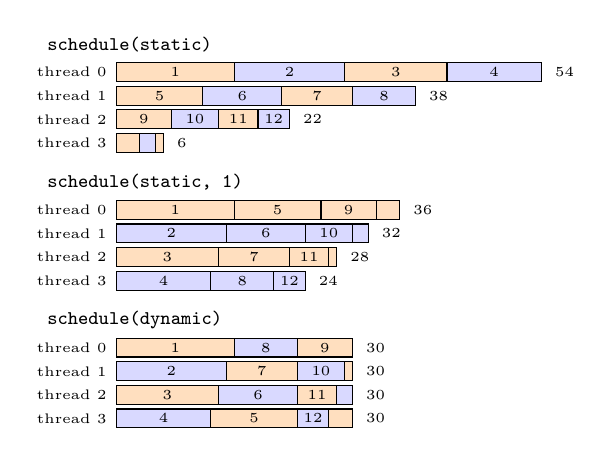
\begin{tikzpicture}[x=1cm, y=1cm]
  \colorlet{c0}{blue!15}
  \colorlet{c1}{orange!25}
  \node[anchor=west, font=\scriptsize] at (-1.0,0.00) {\texttt{schedule(static)}};
  \node[anchor=east, font=\tiny] at (0,-0.35) {thread 0};
  \draw[fill=c1] (0.00,-0.47) rectangle (1.50,-0.23);
  \node[font=\tiny] at (0.75,-0.35) {1};
  \draw[fill=c0] (1.50,-0.47) rectangle (2.90,-0.23);
  \node[font=\tiny] at (2.20,-0.35) {2};
  \draw[fill=c1] (2.90,-0.47) rectangle (4.20,-0.23);
  \node[font=\tiny] at (3.55,-0.35) {3};
  \draw[fill=c0] (4.20,-0.47) rectangle (5.40,-0.23);
  \node[font=\tiny] at (4.80,-0.35) {4};
  \node[anchor=west, font=\tiny] at (5.45,-0.35) {54};
  \node[anchor=east, font=\tiny] at (0,-0.65) {thread 1};
  \draw[fill=c1] (0.00,-0.77) rectangle (1.10,-0.53);
  \node[font=\tiny] at (0.55,-0.65) {5};
  \draw[fill=c0] (1.10,-0.77) rectangle (2.10,-0.53);
  \node[font=\tiny] at (1.60,-0.65) {6};
  \draw[fill=c1] (2.10,-0.77) rectangle (3.00,-0.53);
  \node[font=\tiny] at (2.55,-0.65) {7};
  \draw[fill=c0] (3.00,-0.77) rectangle (3.80,-0.53);
  \node[font=\tiny] at (3.40,-0.65) {8};
  \node[anchor=west, font=\tiny] at (3.85,-0.65) {38};
  \node[anchor=east, font=\tiny] at (0,-0.95) {thread 2};
  \draw[fill=c1] (0.00,-1.07) rectangle (0.70,-0.83);
  \node[font=\tiny] at (0.35,-0.95) {9};
  \draw[fill=c0] (0.70,-1.07) rectangle (1.30,-0.83);
  \node[font=\tiny] at (1.00,-0.95) {10};
  \draw[fill=c1] (1.30,-1.07) rectangle (1.80,-0.83);
  \node[font=\tiny] at (1.55,-0.95) {11};
  \draw[fill=c0] (1.80,-1.07) rectangle (2.20,-0.83);
  \node[font=\tiny] at (2.00,-0.95) {12};
  \node[anchor=west, font=\tiny] at (2.25,-0.95) {22};
  \node[anchor=east, font=\tiny] at (0,-1.25) {thread 3};
  \draw[fill=c1] (0.00,-1.37) rectangle (0.30,-1.13);
  \draw[fill=c0] (0.30,-1.37) rectangle (0.50,-1.13);
  \draw[fill=c1] (0.50,-1.37) rectangle (0.60,-1.13);
  \node[anchor=west, font=\tiny] at (0.65,-1.25) {6};
  \node[anchor=west, font=\scriptsize] at (-1.0,-1.75) {\texttt{schedule(static, 1)}};
  \node[anchor=east, font=\tiny] at (0,-2.10) {thread 0};
  \draw[fill=c1] (0.00,-2.22) rectangle (1.50,-1.98);
  \node[font=\tiny] at (0.75,-2.10) {1};
  \draw[fill=c1] (1.50,-2.22) rectangle (2.60,-1.98);
  \node[font=\tiny] at (2.05,-2.10) {5};
  \draw[fill=c1] (2.60,-2.22) rectangle (3.30,-1.98);
  \node[font=\tiny] at (2.95,-2.10) {9};
  \draw[fill=c1] (3.30,-2.22) rectangle (3.60,-1.98);
  \node[anchor=west, font=\tiny] at (3.65,-2.10) {36};
  \node[anchor=east, font=\tiny] at (0,-2.40) {thread 1};
  \draw[fill=c0] (0.00,-2.52) rectangle (1.40,-2.28);
  \node[font=\tiny] at (0.70,-2.40) {2};
  \draw[fill=c0] (1.40,-2.52) rectangle (2.40,-2.28);
  \node[font=\tiny] at (1.90,-2.40) {6};
  \draw[fill=c0] (2.40,-2.52) rectangle (3.00,-2.28);
  \node[font=\tiny] at (2.70,-2.40) {10};
  \draw[fill=c0] (3.00,-2.52) rectangle (3.20,-2.28);
  \node[anchor=west, font=\tiny] at (3.25,-2.40) {32};
  \node[anchor=east, font=\tiny] at (0,-2.70) {thread 2};
  \draw[fill=c1] (0.00,-2.82) rectangle (1.30,-2.58);
  \node[font=\tiny] at (0.65,-2.70) {3};
  \draw[fill=c1] (1.30,-2.82) rectangle (2.20,-2.58);
  \node[font=\tiny] at (1.75,-2.70) {7};
  \draw[fill=c1] (2.20,-2.82) rectangle (2.70,-2.58);
  \node[font=\tiny] at (2.45,-2.70) {11};
  \draw[fill=c1] (2.70,-2.82) rectangle (2.80,-2.58);
  \node[anchor=west, font=\tiny] at (2.85,-2.70) {28};
  \node[anchor=east, font=\tiny] at (0,-3.00) {thread 3};
  \draw[fill=c0] (0.00,-3.12) rectangle (1.20,-2.88);
  \node[font=\tiny] at (0.60,-3.00) {4};
  \draw[fill=c0] (1.20,-3.12) rectangle (2.00,-2.88);
  \node[font=\tiny] at (1.60,-3.00) {8};
  \draw[fill=c0] (2.00,-3.12) rectangle (2.40,-2.88);
  \node[font=\tiny] at (2.20,-3.00) {12};
  \node[anchor=west, font=\tiny] at (2.45,-3.00) {24};
  \node[anchor=west, font=\scriptsize] at (-1.0,-3.50) {\texttt{schedule(dynamic)}};
  \node[anchor=east, font=\tiny] at (0,-3.85) {thread 0};
  \draw[fill=c1] (0.00,-3.97) rectangle (1.50,-3.73);
  \node[font=\tiny] at (0.75,-3.85) {1};
  \draw[fill=c0] (1.50,-3.97) rectangle (2.30,-3.73);
  \node[font=\tiny] at (1.90,-3.85) {8};
  \draw[fill=c1] (2.30,-3.97) rectangle (3.00,-3.73);
  \node[font=\tiny] at (2.65,-3.85) {9};
  \node[anchor=west, font=\tiny] at (3.05,-3.85) {30};
  \node[anchor=east, font=\tiny] at (0,-4.15) {thread 1};
  \draw[fill=c0] (0.00,-4.27) rectangle (1.40,-4.03);
  \node[font=\tiny] at (0.70,-4.15) {2};
  \draw[fill=c1] (1.40,-4.27) rectangle (2.30,-4.03);
  \node[font=\tiny] at (1.85,-4.15) {7};
  \draw[fill=c0] (2.30,-4.27) rectangle (2.90,-4.03);
  \node[font=\tiny] at (2.60,-4.15) {10};
  \draw[fill=c1] (2.90,-4.27) rectangle (3.00,-4.03);
  \node[anchor=west, font=\tiny] at (3.05,-4.15) {30};
  \node[anchor=east, font=\tiny] at (0,-4.45) {thread 2};
  \draw[fill=c1] (0.00,-4.57) rectangle (1.30,-4.33);
  \node[font=\tiny] at (0.65,-4.45) {3};
  \draw[fill=c0] (1.30,-4.57) rectangle (2.30,-4.33);
  \node[font=\tiny] at (1.80,-4.45) {6};
  \draw[fill=c1] (2.30,-4.57) rectangle (2.80,-4.33);
  \node[font=\tiny] at (2.55,-4.45) {11};
  \draw[fill=c0] (2.80,-4.57) rectangle (3.00,-4.33);
  \node[anchor=west, font=\tiny] at (3.05,-4.45) {30};
  \node[anchor=east, font=\tiny] at (0,-4.75) {thread 3};
  \draw[fill=c0] (0.00,-4.87) rectangle (1.20,-4.63);
  \node[font=\tiny] at (0.60,-4.75) {4};
  \draw[fill=c1] (1.20,-4.87) rectangle (2.30,-4.63);
  \node[font=\tiny] at (1.75,-4.75) {5};
  \draw[fill=c0] (2.30,-4.87) rectangle (2.70,-4.63);
  \node[font=\tiny] at (2.50,-4.75) {12};
  \draw[fill=c1] (2.70,-4.87) rectangle (3.00,-4.63);
  \node[anchor=west, font=\tiny] at (3.05,-4.75) {30};
\end{tikzpicture}
}

      \vspace*{1mm}
      {\small $n = 16$ and four threads. The boxes are the iterations, with lengths proportional to their work. The numbers on the right are the total work of each thread.}
    \end{column}
  \end{columns}
\end{frame}


\begin{frame}
  \frametitle{Amdahl's law}
  \begin{columns}[T]
    \begin{column}{0.5\textwidth}
      \begin{itemize}
        \item Usually only part of a program runs in parallel. If a fraction $f$ of the serial run time is parallelised, the time on $p$ threads is at least $T(p) = T(1) \left[ (1 - f) + f/p \right]$, and the speedup is
          \[ S(p) = \frac{1}{(1 - f) + f/p} \leq \frac{1}{1 - f}. \]
        \item With $f = 0.9$, the speedup can never exceed 10, however many threads there are.
        \item The overheads of the threads and the limited memory bandwidth reduce it further.
      \end{itemize}
    \end{column}

    \begin{column}{0.5\textwidth}
      \centering
      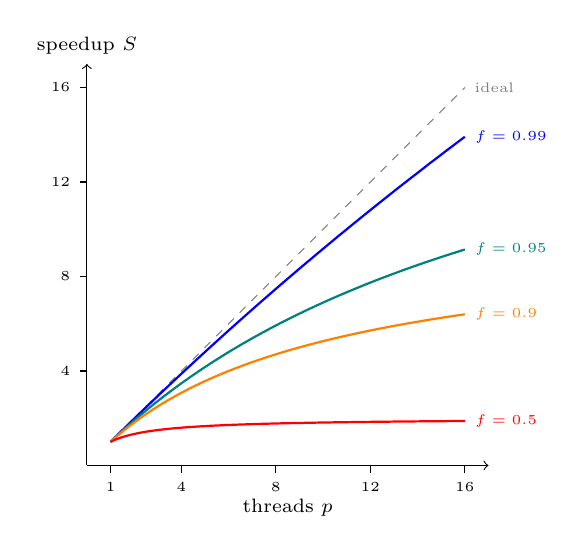
\begin{tikzpicture}[x=0.3cm, y=0.3cm]
        \draw[->] (0,0) -- (17,0);
        \node[font=\scriptsize] at (8.5,-1.8) {threads $p$};
        \draw[->] (0,0) -- (0,17) node[above, font=\scriptsize] {speedup $S$};
        \foreach \x in {1, 4, 8, 12, 16} {
          \draw (\x,0) -- (\x,-0.3) node[below, font=\tiny] {\x};
        }
        \foreach \y in {4, 8, 12, 16} {
          \draw (0,\y) -- (-0.3,\y) node[left, font=\tiny] {\y};
        }
        \draw[gray, dashed] (1,1) -- (16,16) node[right, font=\tiny] {ideal};
        \draw[thick, blue] plot[domain=1:16, samples=60, smooth] (\x, {1/(0.01 + 0.99/\x)}) node[right, font=\tiny] {$f = 0.99$};
        \draw[thick, teal] plot[domain=1:16, samples=60, smooth] (\x, {1/(0.05 + 0.95/\x)}) node[right, font=\tiny] {$f = 0.95$};
        \draw[thick, orange] plot[domain=1:16, samples=60, smooth] (\x, {1/(0.1 + 0.9/\x)}) node[right, font=\tiny] {$f = 0.9$};
        \draw[thick, red] plot[domain=1:16, samples=60, smooth] (\x, {1/(0.5 + 0.5/\x)}) node[right, font=\tiny] {$f = 0.5$};
      \end{tikzpicture}
    \end{column}
  \end{columns}
\end{frame}


\begin{frame}[fragile]
  \frametitle{Common pitfalls}
  \begin{columns}[T]
    \begin{column}{0.5\textwidth}
      \begin{itemize}
        \item \textbf{A forgotten \texttt{private}.} A temporary variable that is shared by default gives a race condition. Use \texttt{default(none)}.
        \item \textbf{An initialised local variable.} \texttt{integer :: k = 0} in a procedure gives \texttt{k} the \texttt{save} attribute, so all the threads share one copy. Assign the value in a separate statement.
        \item \textbf{Too little work.} A team for a short loop, or inside an inner loop, costs more than it saves. Parallelise the outermost loop you can.
      \end{itemize}
    \end{column}

    \begin{column}{0.5\textwidth}
      \begin{itemize}
        \item \textbf{Output inside parallel loops.} The threads queue to print, and the lines come in a random order.
        \item \textbf{False sharing.} Threads that write to neighbouring memory, e.g. \texttt{partial(id)}, slow each other down, because they share a cache line. Use a reduction.
        \item \textbf{Testing with one thread only.} Compare several thread counts with the serial result.
      \end{itemize}

      \begin{lstlisting}
subroutine count_calls()
  integer :: k = 0     ! saved, shared by all threads
  k = k + 1
end subroutine count_calls
      \end{lstlisting}
    \end{column}
  \end{columns}
\end{frame}


\begin{frame}
  \frametitle{More OpenMP}
  \begin{columns}[T]
    \begin{column}{0.5\textwidth}
      \begin{itemize}
        \item The \texttt{do}, \texttt{single}, \texttt{workshare}, and \texttt{sections} constructs, with reductions, are enough for most parallelisation tasks. But OpenMP has much more:
          \begin{itemize}
            \item \texttt{task}: units of work created on the fly, e.g. for recursive algorithms such as tree walks,
            \item \texttt{simd}: vectorisation of a loop on one core,
            \item \texttt{target}: offloading work to a GPU,
            \item locks, nested parallelism, thread affinity\ldots
          \end{itemize}
      \end{itemize}
    \end{column}

    \begin{column}{0.5\textwidth}
      \begin{itemize}
        \item The full list of constructs and clauses is in the OpenMP specification: \url{https://www.openmp.org/specifications/}
        \item Books:
          \begin{itemize}
            \item B. Chapman, G. Jost, R. van der Pas, \emph{Using OpenMP} (MIT Press, 2007),
            \item R. van der Pas, E. Stotzer, C. Terboven, \emph{Using OpenMP -- The Next Step} (MIT Press, 2017),
            \item T. Mattson, Y. He, A. Koniges, \emph{The OpenMP Common Core} (MIT Press, 2019).
          \end{itemize}
      \end{itemize}
    \end{column}
  \end{columns}
\end{frame}


\section{Exercises}

\begin{frame}{Exercise 1: a histogram}
  \begin{block}{Tasks}
    \begin{enumerate}
      \item Write a program that draws $n = 10^7$ random numbers $x$ from \texttt{random\_number}, transforms them to $y = -\ln(1 - x)$, which follows an exponential distribution, and counts the values of $y$ in $[0, 5)$ into 50 bins. Skip the values $y \geq 5$.
      \item Parallelise the counting loop in three ways: with \texttt{critical}, with \texttt{atomic}, and with an array reduction. Check that all three give the same counts as the serial version.
      \item Time the three versions with 1, 2, 4, and 8 threads, and compute the speedups. Which version would you use?
    \end{enumerate}
  \end{block}
\end{frame}


\begin{frame}{Exercise 2: scheduling}
  \begin{block}{Tasks}
    \begin{enumerate}
      \item Write a program that places $N$ points at random in the unit cube, and computes the sum over all the pairs,
        \[ U = -\sum_{i=1}^{N} \sum_{j=i+1}^{N} \frac{1}{|\mathbf{r}_i - \mathbf{r}_j|}, \]
        the potential energy of $N$ unit masses with $G = 1$.
      \item Parallelise the outer loop with a reduction, and time it with $N = 20\,000$ and 1, 2, 4, and 8 threads for \texttt{schedule(static)} and \texttt{schedule(dynamic)}. Use \texttt{schedule(runtime)} and \texttt{OMP\_SCHEDULE}, so that you need to compile only once.
      \item Plot the speedups. Which schedule is faster, and why?
      \item Optional: add \texttt{schedule(static, 1)} and \texttt{schedule(guided)}, and compare with Amdahl's law.
    \end{enumerate}
  \end{block}
\end{frame}


\begin{frame}{Exercise 3: one parallel region}
  \begin{block}{Tasks}
    \begin{enumerate}
      \item Write a program that computes the mean $\mu$, the standard deviation $\sigma$, the minimum, and the maximum of an array of $10^7$ random numbers, all inside \emph{one} parallel region:
        \begin{itemize}
          \item the mean with a \texttt{do} loop and a reduction,
          \item $\sigma$ with a second loop, which needs $\mu$,
          \item and the minimum and the maximum in two \texttt{sections}.
        \end{itemize}
      \item Print the results inside the region with \texttt{single}.
      \item Which barriers are needed? Try removing them with \texttt{nowait}, and explain what happens.
    \end{enumerate}
  \end{block}
\end{frame}

\end{document}
